\documentclass{beamer}
\usepackage{tikz-cd}
\usepackage{tikz}
\renewcommand{\cong}{\simeq}
\newcommand{\ladjoint}{\dashv}
\newcommand{\radjoint}{\vdash}
\newcommand{\<}{\langle}
\renewcommand{\>}{\rangle}
\newcommand{\ndiv}{\hspace{-2pt}\not|\hspace{5pt}}
\newcommand{\cond}{\blacktriangle}
\newcommand{\solid}{\blacksquare}
\newcommand{\ot}{\leftarrow}
\renewcommand{\-}{\text{-}}
\renewcommand{\mapsto}{\leadsto}
\renewcommand{\leq}{\leqslant}
\renewcommand{\geq}{\geqslant}
\renewcommand{\setminus}{\smallsetminus}
\makeatletter
\DeclareRobustCommand{\cev}[1]{%
  {\mathpalette\do@cev{#1}}%
}
\newcommand{\do@cev}[2]{%
  \vbox{\offinterlineskip
    \sbox\z@{$\m@th#1 x$}%
    \ialign{##\cr
      \hidewidth\reflectbox{$\m@th#1\vec{}\mkern4mu$}\hidewidth\cr
      \noalign{\kern-\ht\z@}
      $\m@th#1#2$\cr
    }%
  }%
}
\makeatother

\newcommand{\N}{\mathbb{N}}
\newcommand{\Z}{\mathbb{Z}}
\newcommand{\Q}{\mathbb{Q}}
\newcommand{\R}{\mathbb{R}}
\newcommand{\bbC}{\mathbb{C}}
\NewDocumentCommand{\x}{e{_^}}{%
  \mathbin{\mathop{\times}\displaylimits
    \IfValueT{#1}{_{#1}}
    \IfValueT{#2}{^{#2}}
  }%
}
\NewDocumentCommand{\pushout}{e{_^}}{%
  \mathbin{\mathop{\sqcup}\displaylimits
    \IfValueT{#1}{_{#1}}
    \IfValueT{#2}{^{#2}}
  }%
}
\newcommand{\supp}{\operatorname{supp}}
\newcommand{\im}{\operatorname{im}}
\newcommand{\coker}{\operatorname{coker}}
\newcommand{\id}{\mathrm{id}}
\newcommand{\chara}{\operatorname{char}}
\newcommand{\trdeg}{\operatorname{trdeg}}
\newcommand{\rank}{\operatorname{rank}}
\newcommand{\trace}{\operatorname{tr}}
\newcommand{\length}{\operatorname{length}}
\newcommand{\height}{\operatorname{height}}
\renewcommand{\span}{\operatorname{span}}
\newcommand{\e}{\epsilon}
\newcommand{\p}{\mathfrak{p}}
\newcommand{\q}{\mathfrak{q}}
\newcommand{\m}{\mathfrak{m}}
\newcommand{\n}{\mathfrak{n}}
\newcommand{\calF}{\mathcal{F}}
\newcommand{\calG}{\mathcal{G}}
\newcommand{\calO}{\mathcal{O}}
\newcommand{\F}{\mathbb{F}}
\DeclareMathOperator{\lcm}{lcm}
\newcommand{\gr}{\operatorname{gr}}
\newcommand{\vol}{\mathrm{vol}}

\newcommand{\GL}{\operatorname{GL}}
\newcommand{\SL}{\operatorname{SL}}
\newcommand{\Sp}{\operatorname{Sp}}
\newcommand{\GSp}{\operatorname{GSp}}
\newcommand{\GSpin}{\operatorname{GSpin}}
\newcommand{\opO}{\operatorname{O}}
\newcommand{\SO}{\operatorname{SO}}
\newcommand{\SU}{\operatorname{SU}}
\newcommand{\opU}{\operatorname{U}}
\newcommand{\Spec}{\mathrm{Spec}}
\newcommand{\Spf}{\mathrm{Spf}}
\newcommand{\Spm}{\mathrm{Spm}}
\newcommand{\Spv}{\mathrm{Spv}}
\newcommand{\Spa}{\mathrm{Spa}}
\newcommand{\Spd}{\mathrm{Spd}}
\newcommand{\Proj}{\mathrm{Proj}}
\newcommand{\Gr}{\mathrm{Gr}}
\newcommand{\Hecke}{\mathrm{Hecke}}
\newcommand{\Sht}{\mathrm{Sht}}
\newcommand{\Quot}{\mathrm{Quot}}
\newcommand{\Hilb}{\mathrm{Hilb}}
\newcommand{\Pic}{\mathrm{Pic}}
\newcommand{\Div}{\mathrm{Div}}
\newcommand{\Jac}{\mathrm{Jac}}
\newcommand{\Alb}{\mathrm{Alb}} %albanese variety
\newcommand{\Bun}{\mathrm{Bun}}
\newcommand{\loopspace}{\mathbf{\Omega}}
\newcommand{\suspension}{\mathbf{\Sigma}}
\newcommand{\tangent}{\mathrm{T}} %tangent space
\newcommand{\Eig}{\mathrm{Eig}}

\newcommand{\Ring}{\mathrm{Ring}}
\newcommand{\Cring}{\mathrm{CRing}}
\newcommand{\Alg}{\mathrm{Alg}}
\newcommand{\Leib}{\mathrm{Leib}} %leibniz algebras
\newcommand{\Fld}{\mathrm{Fld}}
\newcommand{\Sets}{\mathrm{Sets}}
\newcommand{\Cat}{\mathrm{Cat}}
\newcommand{\Grp}{\mathrm{Grp}}
\newcommand{\Ab}{\mathrm{Ab}}
\newcommand{\Sch}{\mathrm{Sch}}
\newcommand{\Coh}{\mathrm{Coh}}
\newcommand{\QCoh}{\mathrm{QCoh}}
\newcommand{\Desc}{\mathrm{Desc}}
\newcommand{\Sh}{\mathrm{Sh}}
\newcommand{\Psh}{\mathrm{PSh}}
\newcommand{\Fib}{\mathrm{Fib}}
\renewcommand{\mod}{\-\mathrm{mod}}
\newcommand{\bimod}{\-\mathrm{bimod}}
\newcommand{\Vect}{\mathrm{Vect}}
\newcommand{\Rep}{\mathrm{Rep}}
\newcommand{\Grpd}{\mathrm{Grpd}}
\newcommand{\Arr}{\mathrm{Arr}}
\newcommand{\Esp}{\mathrm{Esp}}
\newcommand{\Ob}{\mathrm{Ob}}
\newcommand{\Mor}{\mathrm{Mor}}
\newcommand{\Mfd}{\mathrm{Mfd}}
%\newcommand{\LR}{\mathrm{LR}}
%\newcommand{\RSpc}{\mathrm{RSpc}}
\newcommand{\Spc}{\mathrm{Spc}}
\newcommand{\Top}{\mathrm{Top}}
\newcommand{\Topos}{\mathrm{Topos}}
\newcommand{\Nil}{\mathfrak{Nil}}
\newcommand{\J}{\mathfrak{J}}
\newcommand{\Stk}{\mathrm{Stk}}
\newcommand{\Pre}{\mathrm{Pre}}
\newcommand{\simp}{\mathbf{\Delta}}
\newcommand{\Ind}{\mathrm{Ind}}
\newcommand{\Pro}{\mathrm{Pro}}
\newcommand{\Mon}{\mathrm{Mon}}
\newcommand{\Comm}{\mathrm{Comm}}
\newcommand{\Fin}{\mathrm{Fin}}
\newcommand{\Assoc}{\mathrm{Assoc}}
\newcommand{\Co}{\mathrm{Co}}
\newcommand{\Comp}{\mathrm{Comp}} %compact hausdorff spaces
\newcommand{\Stone}{\mathrm{Stone}} %stone spaces
\newcommand{\sfExt}{\mathrm{Ext}} %extremely disconnected spaces
\newcommand{\Ouv}{\mathrm{Ouv}}
\newcommand{\Str}{\mathrm{Str}}
\newcommand{\Func}{\mathrm{Func}}
\newcommand{\Crys}{\mathrm{Crys}}
\newcommand{\LocSys}{\mathrm{LocSys}}
\newcommand{\Sieves}{\mathrm{Sieves}}
\newcommand{\pt}{\mathrm{pt}}
\newcommand{\Graphs}{\mathrm{Graphs}}
\newcommand{\Lie}{\mathrm{Lie}}
\newcommand{\Env}{\mathrm{Env}}
\newcommand{\Ho}{\mathrm{Ho}}
\newcommand{\rmD}{\mathrm{D}}
\newcommand{\Cov}{\mathrm{Cov}}
\newcommand{\Frames}{\mathrm{Frames}}
\newcommand{\Locales}{\mathrm{Locales}}
\newcommand{\Span}{\mathrm{Span}}
\newcommand{\Corr}{\mathrm{Corr}}
\newcommand{\Monad}{\mathrm{Monad}}
\newcommand{\Var}{\mathrm{Var}}
\newcommand{\sfN}{\mathrm{N}} %nerve
\newcommand{\Dia}{\mathrm{Dia}}
\newcommand{\co}{\mathrm{co}}
\newcommand{\ev}{\mathrm{ev}}
\newcommand{\bi}{\mathrm{bi}}
\newcommand{\Nat}{\mathrm{Nat}}
\newcommand{\Hopf}{\mathrm{Hopf}}
\newcommand{\Dmod}{\mathrm{D}\mod}
\newcommand{\Perv}{\mathrm{Perv}}
\newcommand{\Sph}{\mathrm{Sph}}
\newcommand{\Moduli}{\mathrm{Moduli}}
\newcommand{\Pseudo}{\mathrm{Pseudo}}
\newcommand{\Lax}{\mathrm{Lax}}
\newcommand{\Strict}{\mathrm{Strict}}
\newcommand{\Opd}{\mathrm{Opd}} %operads
\newcommand{\Shv}{\mathrm{Shv}}
\newcommand{\Char}{\mathrm{Char}} %CharShv = character sheaves
\newcommand{\Huber}{\mathrm{Huber}}
\newcommand{\Tate}{\mathrm{Tate}}
\newcommand{\Ad}{\mathrm{Ad}} %adic spaces
\newcommand{\Perfd}{\mathrm{Perfd}} %perfectoid spaces
\newcommand{\Sub}{\mathrm{Sub}} %subobjects
\newcommand{\Ideals}{\mathrm{Ideals}}
\newcommand{\Isoc}{\mathrm{Isoc}}
\newcommand{\Ban}{\-\mathrm{Ban}} %Banach spaces
\newcommand{\Fre}{\-\mathrm{Fre}} %Frechet spaces
\newcommand{\Ch}{\mathrm{Ch}} %chain complexes
\newcommand{\Mot}{\mathrm{Mot}} %motives
\newcommand{\KL}{\mathrm{KL}} %category of Kazhdan-Lusztig modules
\newcommand{\Pres}{\mathrm{Pres}} %presentable categories

\newcommand{\Aut}{\mathrm{Aut}}
\newcommand{\Inn}{\mathrm{Inn}}
\newcommand{\Out}{\mathrm{Out}}
\newcommand{\frakgl}{\mathfrak{gl}}
\newcommand{\der}{\mathfrak{der}} %derivations on Lie algebras
\newcommand{\inn}{\mathfrak{inn}} %inner derivations
\newcommand{\out}{\mathfrak{out}} %outer derivations
\newcommand{\Stab}{\mathrm{Stab}}
\newcommand{\Cent}{\mathrm{Cent}}
\newcommand{\Conj}{\mathrm{Conj}}
\newcommand{\Gal}{\mathrm{Gal}}
\newcommand{\bfG}{\mathbf{G}} %absolute Galois group
\newcommand{\Frac}{\mathrm{Frac}}
\newcommand{\Ann}{\mathrm{Ann}}
\newcommand{\Val}{\mathrm{Val}}
\newcommand{\Chow}{\mathrm{Chow}}
\newcommand{\Sym}{\mathrm{Sym}}
\newcommand{\End}{\mathrm{End}}
\newcommand{\Mat}{\mathrm{Mat}}
\newcommand{\Diff}{\mathrm{Diff}}
\newcommand{\Autom}{\mathrm{Autom}}

\newcommand{\colim}{\operatorname{colim} \:}
\renewcommand{\lim}{\operatorname{lim} \:}
\newcommand{\toto}{\rightrightarrows}
%\newcommand{\tensor}{\otimes}
\NewDocumentCommand{\tensor}{e{_^}}{%
  \mathbin{\mathop{\otimes}\displaylimits
    \IfValueT{#1}{_{#1}}
    \IfValueT{#2}{^{#2}}
  }%
}
\newcommand{\eq}{\operatorname{eq}}
\newcommand{\coeq}{\operatorname{coeq}}
\newcommand{\Hom}{\mathrm{Hom}}
\newcommand{\Maps}{\mathrm{Maps}}
\newcommand{\Tor}{\mathrm{Tor}}
\newcommand{\Ext}{\mathrm{Ext}}
\newcommand{\Isom}{\mathrm{Isom}}
\newcommand{\stalk}{\mathbf{stalk}}
\newcommand{\RKE}{\operatorname{RKE}}
\newcommand{\LKE}{\operatorname{LKE}}
\newcommand{\oblv}{\mathbf{oblv}}
\newcommand{\const}{\mathbf{const}}
%\newcommand{\forget}{\mathbf{forget}}
\newcommand{\adrep}{\mathbf{ad}} %adjoint representation
\newcommand{\NL}{\mathbf{NL}} %naive cotangent complex
\newcommand{\bfL}{\mathbf{L}} %cotangent complex
\newcommand{\pr}{\operatorname{pr}}
\newcommand{\Der}{\mathbf{Der}}
\newcommand{\Frob}{\mathrm{Frob}} %Frobenius
\newcommand{\frob}{\mathrm{frob}} %trace of Frobenius
\newcommand{\bfpt}{\mathbf{pt}}
\newcommand{\bfloc}{\mathbf{loc}}
\newcommand{\1}{\mathbbm{1}}
\newcommand{\2}{\mathbbm{2}}
\newcommand{\Jet}{\mathbf{Jet}}
\newcommand{\Split}{\mathbf{Split}}
\newcommand{\Sq}{\mathbf{Sq}}
\newcommand{\Zero}{\mathbf{Z}}
\newcommand{\SqZ}{\Sq\Zero}
\newcommand{\frakLie}{\mathfrak{Lie}}
\newcommand{\y}{\mathbf{y}} %yoneda
\newcommand{\Sm}{\mathrm{Sm}}
\newcommand{\AJ}{\mathrm{AJ}} %abel-jacobi map
\newcommand{\act}{\mathrm{act}}
\newcommand{\ram}{\mathrm{ram}} %ramification index
\newcommand{\inv}{\mathrm{inv}}

\newcommand{\bbU}{\mathbb{U}}
\newcommand{\V}{\mathbb{V}}
\newcommand{\U}{\mathrm{U}}
\newcommand{\rmI}{\mathrm{I}} %augmentation ideal
\newcommand{\bfV}{\mathbf{V}}
\newcommand{\C}{\mathcal{C}}
\newcommand{\D}{\mathcal{D}}
\newcommand{\T}{\mathbf{T}} %Tate modules
\newcommand{\calM}{\mathcal{M}}
\newcommand{\calN}{\mathcal{N}}
\newcommand{\calP}{\mathcal{P}}
\newcommand{\calQ}{\mathcal{Q}}
\newcommand{\A}{\mathbb{A}}
\renewcommand{\P}{\mathbb{P}}
\newcommand{\calL}{\mathcal{L}}
\newcommand{\E}{\mathcal{E}}
\renewcommand{\H}{\mathbf{H}}
\newcommand{\calX}{\mathcal{X}}
\newcommand{\calY}{\mathcal{Y}}
\newcommand{\calZ}{\mathcal{Z}}
\newcommand{\scrX}{\mathscr{X}}
\newcommand{\scrY}{\mathscr{Y}}
\newcommand{\scrZ}{\mathscr{Z}}
\newcommand{\calA}{\mathcal{A}}
\newcommand{\calB}{\mathcal{B}}
\newcommand{\sfT}{\mathrm{T}}
\renewcommand{\S}{\mathcal{S}}
\newcommand{\B}{\mathbb{B}}
\newcommand{\bbD}{\mathbb{D}}
\newcommand{\G}{\mathbb{G}}
\newcommand{\horn}{\mathbf{\Lambda}}
\renewcommand{\L}{\mathbb{L}}
\renewcommand{\a}{\mathfrak{a}}
\renewcommand{\b}{\mathfrak{b}}
\renewcommand{\t}{\mathfrak{t}}
\renewcommand{\r}{\mathfrak{r}}
\newcommand{\bbX}{\mathbb{X}}
\newcommand{\g}{\mathfrak{g}}
\newcommand{\h}{\mathfrak{h}}
\renewcommand{\k}{\mathfrak{k}}
\newcommand{\del}{\partial}
\newcommand{\bbE}{\mathbb{E}}
\newcommand{\scrO}{\mathscr{O}}
\newcommand{\bbO}{\mathbb{O}}
\newcommand{\scrA}{\mathscr{A}}
\newcommand{\scrB}{\mathscr{B}}
\newcommand{\scrF}{\mathscr{F}}
\newcommand{\scrG}{\mathscr{G}}
\newcommand{\scrM}{\mathscr{M}}
\newcommand{\scrN}{\mathscr{N}}
\newcommand{\scrP}{\mathscr{P}}
\newcommand{\frakS}{\mathfrak{S}}
\newcommand{\calI}{\mathcal{I}}
\newcommand{\calJ}{\mathcal{J}}
\newcommand{\calK}{\mathcal{K}}
\newcommand{\scrV}{\mathscr{V}}
\newcommand{\bbS}{\mathbb{S}}
\newcommand{\scrH}{\mathscr{H}}
\newcommand{\bfB}{\mathbf{B}}
\newcommand{\W}{\mathbf{W}}
%\newcommand{\bfA}{\mathbf{A}}
\renewcommand{\O}{\mathbb{O}}
\newcommand{\calV}{\mathcal{V}}
\newcommand{\scrR}{\mathscr{R}} %radical
\newcommand{\rmZ}{\mathrm{Z}} %centre of algebra
\newcommand{\bfGamma}{\mathbf{\Gamma}}
\newcommand{\scrU}{\mathscr{U}}
\newcommand{\rmW}{\mathrm{W}} %Weil group

\newcommand{\aff}{\mathrm{aff}}
\newcommand{\ft}{\mathrm{ft}} %finite type
\newcommand{\fp}{\mathrm{fp}} %finite presentation
\newcommand{\aft}{\mathrm{aft}}
\newcommand{\lft}{\mathrm{lft}}
\newcommand{\laft}{\mathrm{laft}}
\newcommand{\cmpt}{\mathrm{cmpt}}
\newcommand{\qc}{\mathrm{qc}}
\newcommand{\qs}{\mathrm{qs}}
\newcommand{\lcmpt}{\mathrm{lcmpt}}
%\newcommand{\conv}{\mathrm{conv}}
\newcommand{\red}{\mathrm{red}}
\newcommand{\fin}{\mathrm{fin}}
\newcommand{\gen}{\mathrm{gen}}
\newcommand{\petit}{\mathrm{petit}}
\newcommand{\gros}{\mathrm{gros}}
\newcommand{\loc}{\mathrm{loc}}
\newcommand{\glob}{\mathrm{glob}}
\newcommand{\ringed}{\mathrm{ringed}}
\newcommand{\qcoh}{\mathrm{qcoh}}
\newcommand{\cl}{\mathrm{cl}}
\newcommand{\et}{\mathrm{\acute{e}t}}
\newcommand{\fet}{\mathrm{f\acute{e}t}}
\newcommand{\profet}{\mathrm{prof\acute{e}t}}
\newcommand{\proet}{\mathrm{pro\acute{e}t}}
\newcommand{\Zar}{\mathrm{Zar}}
\newcommand{\fppf}{\mathrm{fppf}}
\newcommand{\fpqc}{\mathrm{fpqc}}
\newcommand{\smooth}{\mathrm{sm}}
\newcommand{\sh}{\mathrm{sh}}
\newcommand{\op}{\mathrm{op}}
\newcommand{\open}{\mathrm{open}}
\newcommand{\closed}{\mathrm{closed}}
\newcommand{\geom}{\mathrm{geom}}
\newcommand{\alg}{\mathrm{alg}}
\newcommand{\sober}{\mathrm{sober}}
\newcommand{\dR}{\mathrm{dR}}
\newcommand{\rad}{\mathrm{rad}}
\newcommand{\discrete}{\mathrm{discrete}}
%\newcommand{\add}{\mathrm{add}}
%\newcommand{\lin}{\mathrm{lin}}
\newcommand{\Krull}{\mathrm{Krull}}
\newcommand{\qis}{\mathrm{qis}} %quasi-isomorphism
\newcommand{\ho}{\mathrm{ho}} %homotopy equivalence
\newcommand{\sep}{\mathrm{sep}}
\newcommand{\unr}{\mathrm{unr}}
\newcommand{\tame}{\mathrm{tame}}
\newcommand{\wild}{\mathrm{wild}}
\newcommand{\nil}{\mathrm{nil}}
\newcommand{\defm}{\mathrm{defm}}
\newcommand{\Art}{\mathrm{Art}}
\newcommand{\Noeth}{\mathrm{Noeth}}
\newcommand{\affd}{\mathrm{affd}}
%\newcommand{\adic}{\mathrm{adic}}
\newcommand{\pre}{\mathrm{pre}}
\newcommand{\perf}{\mathrm{perf}}
\newcommand{\perfd}{\mathrm{perfd}}
\newcommand{\rat}{\mathrm{rat}}
\newcommand{\cont}{\mathrm{cont}}
\newcommand{\dg}{\mathrm{dg}}
\newcommand{\almost}{\mathrm{a}}
%\newcommand{\stab}{\mathrm{stab}}
\newcommand{\heart}{\heartsuit}
\newcommand{\proj}{\mathrm{proj}}
\newcommand{\qproj}{\mathrm{qproj}}
\newcommand{\pd}{\mathrm{pd}}
\newcommand{\crys}{\mathrm{crys}}
\newcommand{\prisma}{\mathrm{prisma}}
\newcommand{\FF}{\mathrm{FF}}
\newcommand{\sph}{\mathrm{sph}}
\newcommand{\lax}{\mathrm{lax}}
\newcommand{\weak}{\mathrm{weak}}
\newcommand{\strict}{\mathrm{strict}}
\newcommand{\mon}{\mathrm{mon}}
\newcommand{\sym}{\mathrm{sym}}
\newcommand{\lisse}{\mathrm{lisse}}
\newcommand{\an}{\mathrm{an}}
\newcommand{\ad}{\mathrm{ad}}
\newcommand{\sch}{\mathrm{sch}}
\newcommand{\rig}{\mathrm{rig}}
\newcommand{\pol}{\mathrm{pol}}
\newcommand{\plat}{\mathrm{flat}}
\newcommand{\proper}{\mathrm{proper}}
\newcommand{\compl}{\mathrm{compl}}
\newcommand{\non}{\mathrm{non}}
\newcommand{\access}{\mathrm{access}}
\newcommand{\comp}{\mathrm{comp}}
\newcommand{\tstructure}{\mathrm{t}} %t-structures
\newcommand{\pure}{\mathrm{pure}} %pure motives
\newcommand{\mixed}{\mathrm{mixed}} %mixed motives
\newcommand{\num}{\mathrm{num}} %numerical motives
\newcommand{\ess}{\mathrm{ess}}
\newcommand{\topological}{\mathrm{top}}
\newcommand{\convex}{\mathrm{cv}}
\newcommand{\ab}{\mathrm{ab}} %abelian extensions
\newcommand{\surj}{\mathrm{surj}} %coverage on sets generated by surjections
\newcommand{\eff}{\mathrm{eff}} %effective Cartier divisors
\newcommand{\Weil}{\mathrm{Weil}} %weil divisors
\newcommand{\lex}{\mathrm{lex}}
\newcommand{\rex}{\mathrm{rex}}
\newcommand{\AR}{\mathrm{A\-R}}

%prism custom command
\usepackage{relsize}
\usepackage[bbgreekl]{mathbbol}
\usepackage{amsfonts}
\DeclareSymbolFontAlphabet{\mathbb}{AMSb} %to ensure that the meaning of \mathbb does not change
\DeclareSymbolFontAlphabet{\mathbbl}{bbold}
\newcommand{\prism}{{\mathlarger{\mathbbl{\Delta}}}}

%Information to be included in the title page:
\title{Geometric unramified abelian class field theory for curves\\and\\The Langlands Correspondence for $\GL_1$ over global function fields over finite fields}
\author{Dat Minh Ha (UCID: 30067407)}
\institute{Department of Mathematics and Statistics\\University of Calgary}
\date{March 23rd 2022}

\begin{document}

    \frame{\titlepage}
    
    \begin{frame}
        \begin{figure}[H]
            \centering
            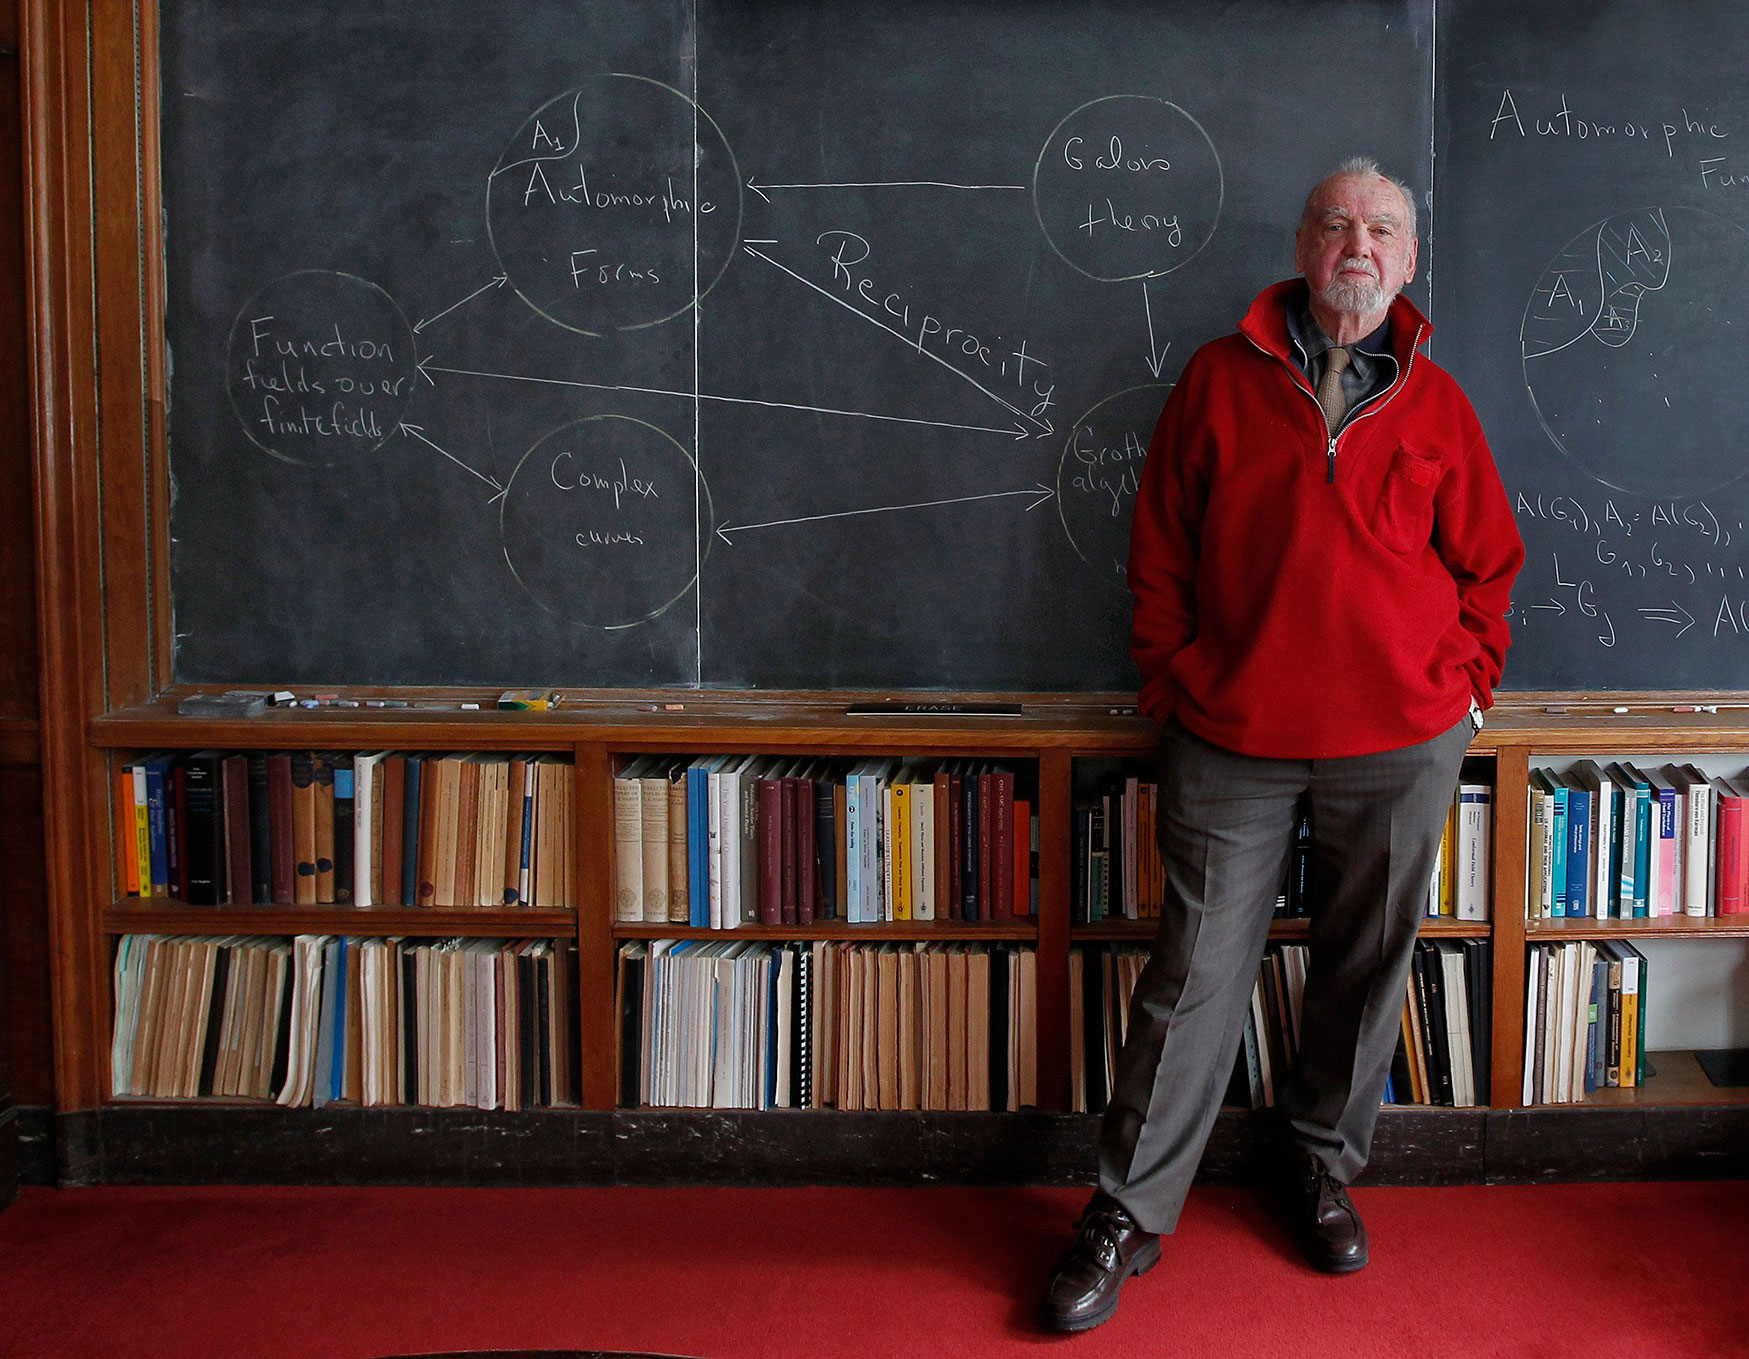
\includegraphics[width=10cm,height=10cm,keepaspectratio]{Proposal, timeline, and presentation/robert_langlands.jpg}
            \caption{Robert Langlands: the biggest job-provider in mathematics since Hilbert}
            \label{fig: robert_langlands}
        \end{figure}
    \end{frame}
    
    \begin{frame}{The Langlands Correspondence ?}
        \frametitle{}
        \begin{itemize}
            \item The Langlands Programme is a web of deep conjectures and theorems that together seek a unification of the two large pillars of modern number theory, \textbf{Galois groups} and \textbf{automorphic forms}. In more general terms, one can say that the Langlands Programme seek to bring algebraic and analytic number theory together.
            \item Central to the Programme is the Langlands Correspondence, which takes the form of a (conjectural) bijection of the following sort:    
                $$\left\{\text{Galois representations}\right\} \cong \left\{\text{Automorphic forms}\right\}$$
        \end{itemize}
    \end{frame}
    
    \begin{frame}{The plan}
        I shall attempt to explain the ingredients at play, as well as how this correspondence relates to my project.
    \end{frame}
    
    \begin{frame}{Galois representations ?}
        \begin{itemize}
            \item Groups encode symmetries of spaces, so are best understood via their actions. We understand linear algebra over fields very well, so a natural method for studying groups $G$ is looking at their \textbf{linear representations}, i.e. homomorphisms:
                $$\rho: G \to \Aut(V)$$
            \item Infinite-dimensional vector spaces are nasty, so we restrict our attention to finite-dimensional representations.
            \item (Absolute) Galois groups are no different, so one studies Galois groups via so-called \textbf{Galois representations}:
                $$\rho: \Gal(\bar{K}/K) \to \GL_n(E)$$
        \end{itemize}
    \end{frame}
    
    \begin{frame}{Back to the Langlands Correspondence ...}
        
        \begin{itemize}
            \item The Modularity Theorem (over $\Q$)\footnote{Which implies Fermat's Last Theorem!} is a special case of the Langlands Correspondence, namely the case concerning $2$-dimensional representations of $\Gal(\bar{\Q}/\Q)$. It tells us that to every elliptic curve one can associate a unique modular form of a certain kind\footnote{Which can be thought of as a special kind of automorphic form.}. The Langlands Programme therefore benefits the study of elliptic curves for say, cryptography, greatly.
            \item We are interested in something very similar (at least in spirit), albeit much simpler.
        \end{itemize}
    \end{frame}
    
    \begin{frame}{Automorphic forms}
        On the other side of the Langlands Correspondence are \textbf{automorphic forms}. These are - in rough terms - functions of great arithmetic significance and close ties to entities such as Eisenstein series and L-functions (of which $\zeta$-functions are special cases), and as such are of interest when one tries to answer questions regarding patterns that prime numbers as a whole exhibit, such as analogues of the Riemann Hypothesis/Conjecture.
    \end{frame}
    
    \begin{frame}{Automorphic forms}
         We focus on automorphic forms instead of L-functions (and so on) because doing so gives us access to the powerful tools of harmonic analysis (Fourier analysis for topologically groups\footnote{Hopefully, we will be able to figure out what happens over non-abelian topological groups like $\GL_n$!} more general than the circle group $\GL_1$). 
    \end{frame}
    
    \begin{frame}{Function fields}
        Let $k$ be any field. Then there is an equivalence of categories:
            $$\{\text{Field extensions $K/k$ of ft. and $k$-alg. hom.}\}^{\op}$$
            $$\cong$$
            $$\{\text{Varieties $X/k$ and dominant rational maps}\}$$
    \end{frame}
    
    \begin{frame}{Function fields}
        For curves, it's even better:
            $$\{\text{Field extensions $K/k$ of $\trdeg = 1$ and $k$-alg. hom.}\}^{\op}$$
            $$\cong$$
            $$\{\text{Curves $X/k$ and dominant rational maps}\}$$
            $$\cong$$
            $$\{\text{Non-singular projective curves $X/k$ and dominant rational maps}\}$$
    \end{frame}
    
    \begin{frame}{Function fields}
        \begin{itemize}
            \item Understanding (smooth) curves $X$ will help us understand algebraic extensions of the \textbf{global function field} $K_X$. E.g. the function field of $\P^1_k$ (for any field $k$) is actually $k(t)$ itself.
            \item When we say that a field $K$ is \textbf{global}, we roughly mean that it behaves similarly to fields like $\Q$, $\F_p(t)$, or $\bbC(t)$, in the sense that for each of them, there exists a set of ultranorms $v$, such that the topological completions with respect to all of them are locally compact Hausdorff non-discrete topological fields such as $\R, \Q_p$, $\F_p(\!(t)\!)$, or $\bbC(\!(t)\!)$.
        \end{itemize}
    \end{frame}
    
    \begin{frame}{What we are after ...}
        What we want is the Langlands Correspondence for $\GL_1$ over algebraic extensions $K/\F_p(t)$, which reads:
            $$\left\{\text{$1$-dimensional Galois representations of $\Gal(\bar{K}/K)$}\right\}$$
            $$\cong$$
            $$\left\{\text{Autmorphic forms attached to $\GL_1(K)$}\right\}$$
        On the streets this is also known as the \textbf{Global Artin Reciprocity Law}, the crowning jewel of classical global class field theory.
    \end{frame}
    
    \begin{frame}{What is actually being done ?}
        \begin{itemize}
            \item Obtaining the Global Artin Reciproty Law in the traditional manner (e.g. via Galois cohomology) is no small feat, and while the result is very impressive and important, it is not at all obvious how we might make the jump from $\GL_1$ to matrix groups of higher dimensions.
            \item To that end, we construct a "toy model" of the Reciprocity Law - much like how one might construct mathematical models in order to derive predictions in the natural sciences - via a process known as "categorification".
        \end{itemize}
    \end{frame}
    
    \begin{frame}{Geometric vs. function-theoretic Langlands Correspodences}
        \begin{itemize}
            \item The geometric correspondence takes the form:
                $$\left\{\text{$\ell$-adic sheaves/perverse sheaves/D-modules/etc. on $X$}\right\}$$
                $$\cong$$
                $$\left\{\text{Hecke eigensheaves on $\Bun_{\GL_1}(X)$}\right\}$$
            \item Compare this with the function-theoretic correspondence:
                $$\left\{\text{$1$-dimensional Galois representations of $\Gal(\bar{K}/K)$}\right\}$$
                $$\cong$$
                $$\left\{\text{Autmorphic forms attached to $\GL_1(K)$}\right\}$$
        \end{itemize}
    \end{frame}

\end{document}